% !TeX document-id = {c974e6b9-54de-4014-ab33-a7c58a019f7c}
% !TeX program = xelatex
% !TeX TXS-program:bibliography = txs:///biber

\documentclass[11pt]{article}

\usepackage[margin=1in]{geometry}
\usepackage{graphicx}
\usepackage[style=ieee,backend=biber,maxbibnames=99]{biblatex}
\usepackage{amsmath}
\usepackage{hyperref}
\usepackage{cleveref}
\usepackage{siunitx}
\usepackage{fontspec}
\usepackage{unicode-math}
%\setmainfont{TeX Gyre Pagella}
\setmathfont{Asana Math}


\addbibresource{02_rocpicker.bib}

\title{Finding error bands for a ROC curve}
\author{Heshy Roskes}
\date{}

\newcommand{\xdot}{\dot{x}}
\newcommand{\ydot}{\dot{y}}
\newcommand{\Xdot}{\dot{X}}
\newcommand{\Ydot}{\dot{Y}}
\newcommand{\Xdotdot}{\ddot{X}}
\newcommand{\AUC}{AUC}
\begin{document}
\maketitle

\begin{center}

\includegraphics[width=0.4\textwidth]{logo.png}
\end{center}

\section{Introduction}

We want to solve the following problem:

We have a set of samples characterized by a parameter \(t\) (for example, density of CD8+FoxP3+-like neighborhoods).  They are divided into two groups (responders and non-responders to anti-PD1).  We expect that one group (responders) will have a higher \(t\) than the other group (non-responders) and want to illustrate this using a ROC curve.  How can we estimate the uncertainties on the ROC curve?

One source of uncertainty is the statistics of our sample set.  We don't know the real distribution of \(t\) for the two groups; we only know the distribution for the samples we have.

Each sample's \(t\) measurement also comes with its own statistical and systematic uncertainties.  The systematic uncertainties might also be correlated between all the samples or between a subset of the samples (and this subset could include some samples from both groups).

At this point I want to address the first source of uncertainty.  I think the method will extend nicely to sample-wise uncertainties too.

\section{Previous approaches}

Many methods \autocite{roc_kerekes} deal with individual points on the ROC curve without taking their correlations into account.  There is a paper from Tilbury 25 years ago \autocite{roc_tilbury} that does something similar to what we're doing here, but in a \emph{very} computationally expensive way, with only three points.  It would scale terribly to a ROC curve with more points.  The authors note that one of the computations done for that paper ``ran for over a month on a powerful Unix workstation''.  A quarter century later, it would run faster, but the method still scales poorly with the number of points on the ROC curve.

A more recent paper and accompanying R package \autocite{roc_fernandez} includes three methods of computing confidence intervals on a ROC curve, using various assumptions and approximations.

In any case, none of these papers considered any uncertainties other than the binomial statistical uncertainty on the number of samples.  We want a method that can generalize to sample-wise uncertainties, which can include statistical uncertainties on counts and any kind of systematic uncertainty.

There is something similar for Kaplan-Meier curves \autocite{kaplanmeier_sachs}.  It correctly considers the whole curve as a unit, but also doesn't include systematic uncertainties.

\section{Statistical uncertainty}\label{sec:stat}

A ROC curve is a plot of \(x(t), y(t)\), where \(x(t)\) is the cumulative density function (CDF) of \(t\) for one group (non-responders) and \(y(t)\) is the CDF for the other group (responders).  The derivatives, \(\xdot(t)\) and \(\ydot(t)\), give the probability density functions (PDFs) for the two groups.   We want to find a probability distribution for the ``true'' \(x\) and \(y\) distributions, given our observed data.

Our observed data for the two groups have CDFs \(X(t), Y(t)\) and PDFs \(\Xdot(t), \Ydot(t)\).  In reality, \(\Xdot\) and \(\Ydot\) are going to be sums of delta functions, while the true probability distributions \(\xdot\) and \(\ydot\) are unknown, continuous distributions.  In order to make the problem feasible, we have to make some assumptions on the form of \(\xdot\) and \(\ydot\).  The current package includes three implementations.

\subsection{Discrete points}\label{sec:discrete}

In the first implementation, we consider \(\Xdot\) and \(\Ydot\) as discrete.  Furthermore, we assume that the true probability distributions \(\xdot\) and \(\ydot\) are also sums of delta functions, where \(\xdot\) only has nonzero probability where \(\Xdot\) does and \(\ydot\) only has nonzero probability where \(\Ydot\) does, but possibly with different relative weights.  This is equivalent to assuming that all future patients will be identical to one of the current ones.  Formally,
\begin{align}
\begin{aligned}
\Xdot(t)&=\sum_n \mathscr{X}_n \delta(t-t_n) \\
\Ydot(t)&=\sum_r \mathscr{Y}_r \delta(t-t_r) \\
\xdot(t)&=\sum_n \mathscr{x}_n \delta(t-t_n) \\
\ydot(t)&=\sum_r \mathscr{y}_r \delta(t-t_r) \\
\end{aligned}
\label{eq:roc-from-delta-functions}
\end{align}
The indices \(n\) and \(r\) index the non-responders and responders, \(\mathscr{X}_n\) and \(\mathscr{Y}_r\) are the numbers of non-responders and responders with \(t=t_n\) or \(t=t_r\), and \(\mathscr{x}_n\) and \(\mathscr{y}_r\) are the fractions of non-responders and responders with \(t=t_n\) or \(t=t_r\) in the true probability distribution.

\subsubsection{The most likely \texorpdfstring{\(\mathscr{x}\)}{x} and \texorpdfstring{\(\mathscr{y}\)}{y}}\label{sec:discrete_unconstrained}

Given \(\mathscr{x}_n\) and \(\mathscr{y}_r\), the probability to observe our data \((\mathscr{X}_n, \mathscr{Y}_r)\) is
\begin{equation}
\ln{L}=-\sum_{n}\mathscr{X}_n\ln{\mathscr{x}_n}-\sum_{r}\mathscr{Y}_r\ln{\mathscr{y}_r}
\label{eq:discrete_loglikelihood}
\end{equation}
We want to maximize this likelihood with the constraint
\begin{align}
\begin{aligned}
\sum_n{\mathscr{x}_n}&=1 \\
\sum_r{\mathscr{y}_r}&=1
\end{aligned}
\label{eq:discrete_normalization}
\end{align}
We get
\begin{align}
\begin{aligned}
\frac{\partial}{\partial \mathscr{x}_n}(\ln{L} + \lambda_x \sum_n {\mathscr{x}_n} + \lambda_y \sum_r{\mathscr{y}_r})&=0 \\
-\frac{\mathscr{X}_n}{\mathscr{x}_n}+\lambda_x&=0 \\
\end{aligned}
\end{align}
The result is
\begin{align}
\begin{aligned}
\mathscr{x}_n&=\frac{\mathscr{X}_n}{\sum_{n^\prime}\mathscr{X}_{n^\prime}} \\
\mathscr{y}_r&=\frac{\mathscr{Y}_r}{\sum_{r^\prime}\mathscr{Y}_{r^\prime}}
\end{aligned}
\end{align}
In other words, the most likely probability distribution given our data is the probability distribution that we observe in the data.  No surprise.

\subsubsection{Likelihood scan for AUC}\label{sec:discrete_likelihood_scan}

One metric that is commonly used to assess the power of \(t\) to separate the two groups is the AUC, or area under the ROC curve.  Using our notation, this is
\begin{align}
	\begin{aligned}
		\AUC&=\int_{0}^{1}ydx\\
		&=\int_{-\infty}^{\infty}y\xdot dt \label{eq:AUC}
	\end{aligned}
\end{align}
We want to find a way to estimate the error on the AUC\@.  To do this, we will use a likelihood scan:
\begin{enumerate}
	\item Fix the AUC to a particular value
	\item Of all possible curves \(x(t), y(t)\) that satisfy \cref{eq:AUC}, find the one that is most likely given our data
	\item Evaluate its negative log likelihood (\cref{eq:discrete_loglikelihood})
	\item Plot the best fit negative log likelihood as a function of the AUC\@.  The most likely AUC is the one that minimizes this log likelihood, which we found in \cref{sec:discrete_unconstrained}, and we subtract this minimum to obtain \(-2\Delta\ln{L}\).  The 68\% confidence interval is where \(-2\Delta\ln{L}<1\), and the 95\% confidence interval is where \(-2\Delta\ln{L}<3.84\).
\end{enumerate}

Our implementation uses \texttt{scipy.optimize.minimize} with \texttt{method=SLSQP}.  We introduce an explicit constraint for the AUC\@.  For the normalizations (\cref{eq:discrete_normalization}), we do not introduce a constraint, but instead apply the normalization internally before calculating the log-likelihood and AUC\@.  In our tests, this minimization converges reliably and instantaneously.

\subsubsection{Example}

In this simple example, we have 7 responders \(t_r=(1, 1, 2, 2, 3, 9, 10)\) and 14 non-responders \(t_n=(2, 3, 3, 4, 6, 8, 9, 10, 10, 10, 10, 11, 12, 13)\).  The ROC curve is shown in \cref{fig:exampledata_discrete} (left).  The middle plot shows a likelihood scan for the AUC\@.  The right hand plot shows the ROC curves corresponding to the 68\% and 95\% AUCs.

It is important to note that there is not just one up and down variation of the curve for a given confidence level, and any choice is only an illustration.  In other words, the edges of the error bands in \cref{fig:exampledata_discrete} (right) are \emph{not} the only possible ROC curves that mark the boundaries of the 68\% and 95\% regions.  They are only the 68\% and 95\% ROC curves with AUCs most distant from the nominal AUC, and are therefore informative for illustration.  Other packages, such as \autocite{roc_fernandez}, have a different method of illustrating the uncertainty band for the whole curve.

\begin{figure}
	\begin{center}
		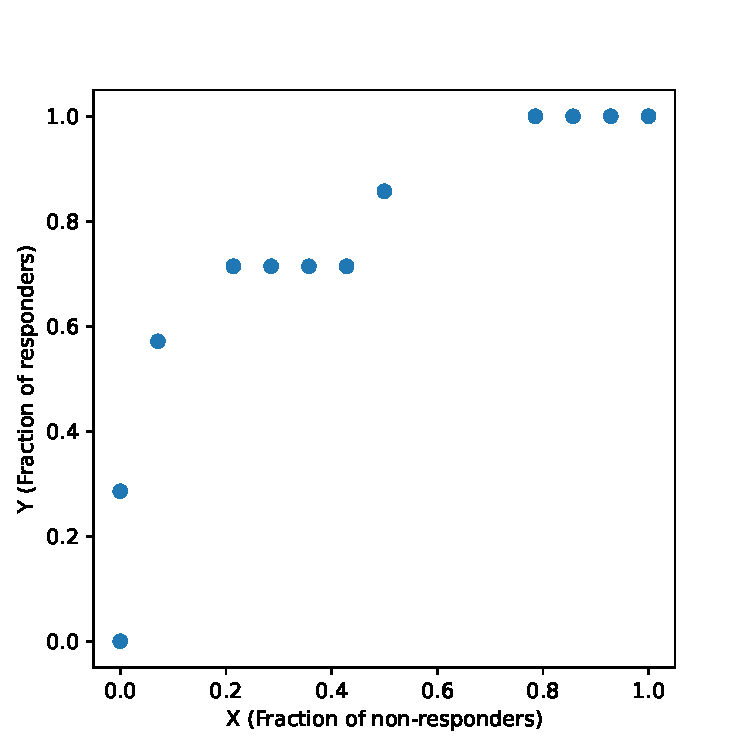
\includegraphics[width=0.32\textwidth]{discrete_exampleroc.pdf}
		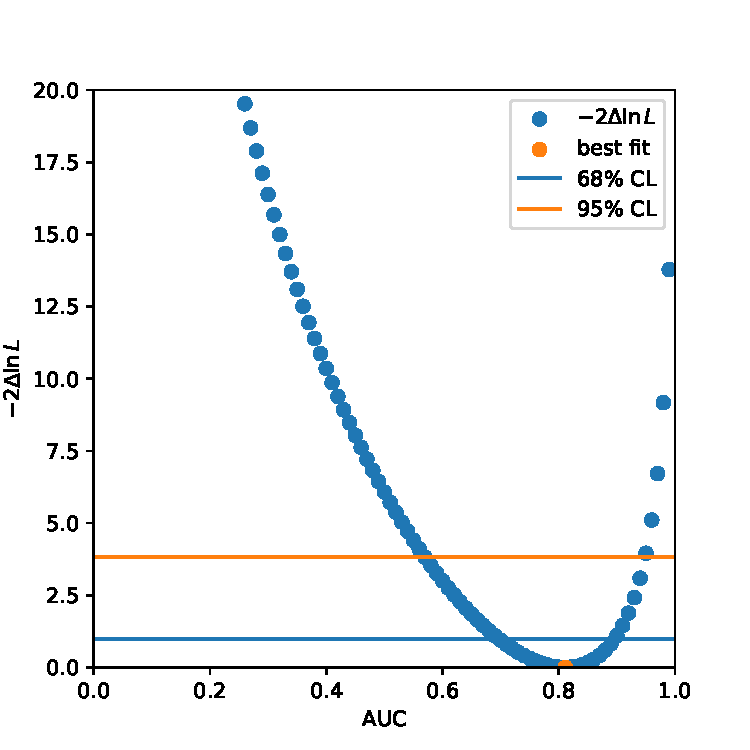
\includegraphics[width=0.32\textwidth]{discrete_scan.pdf}
		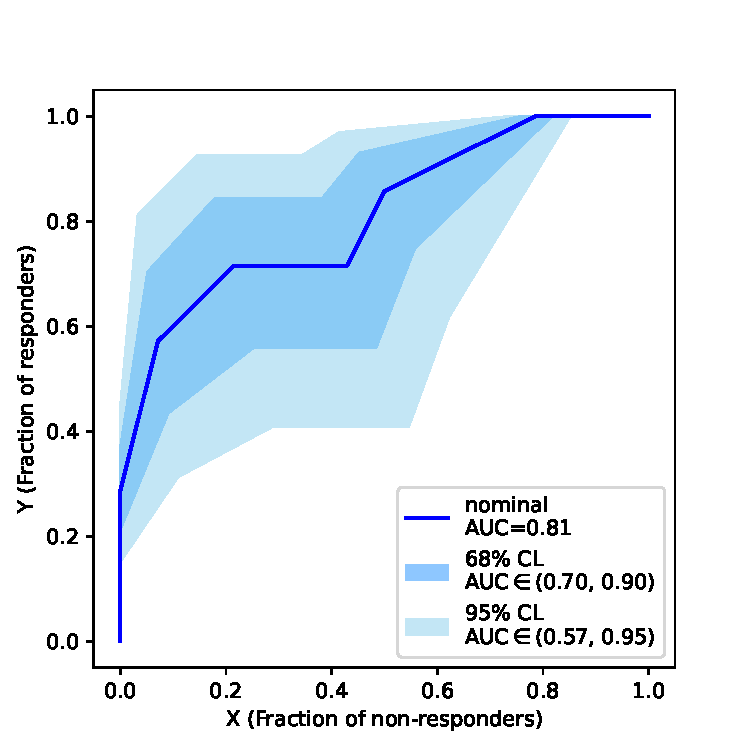
\includegraphics[width=0.32\textwidth]{discrete_exampleroc_errors.pdf}
		\caption{Plots for the example distributions. Left: The ROC curve. Middle: The likelihood scan. Right: The best-fitted ROC curve, with 68\% and 95\% error bands indicating the best-fitted ROC curves with AUCs at the edges of the 68\% and 95\% CL regions from the likelihood scan.\label{fig:exampledata_discrete}}
	\end{center}
\end{figure}

\subsection{Continuous distributions}\label{sec:lagrangian}

Our second implementation uses \(\Xdot\) and \(\Ydot\) as continuous, and in this way we use continuous distributions in our tests.  They are normalized so that
\begin{align}
\begin{aligned}
X(-\infty)=Y(-\infty)&=0 \\
X(+\infty)&=n_X \\
Y(+\infty)&=n_Y
\end{aligned}
\end{align}

The probability density to observe a non-responder or responder at \(t_i\) is just \(\xdot(t)\) or \(\ydot(t)\), and the log likelihood is \(\ln{\xdot(t)}\) or \(\ln{\ydot(t)}\).  Summing this log likelihood over our whole observed dataset, we get
\begin{equation}
	-2\ln{L}=-2\int_{-\infty}^{\infty}dt\left(\Xdot(t)\ln{\xdot(t)}+\Ydot(t)\ln{\ydot(t)}\right).
	\label{eq:loglikelihood}
\end{equation}
We want to find \(x(t)\) and \(y(t)\), given \(\Xdot(t)\) and \(\Ydot(t)\).  Note that we have the boundary conditions
\begin{align}
\begin{aligned}
	x(-\infty)=y(-\infty)&=0\\
	x(+\infty)=y(+\infty)&=1
\end{aligned}
\label{eq:boundaryconditions}
\end{align}

To do find \(x\) and \(y\), we minimize \cref{eq:loglikelihood}.  Our Lagrangian is
\begin{equation}
	\mathcal{L}[x,\xdot,y,\ydot,t]=-2\left(\Xdot(t)\ln{\xdot(t)}+\Ydot(t)\ln{\ydot(t)}\right),
	\label{eq:lagrangian}
\end{equation}
and the Euler-Lagrange equations are
\begin{align}
\begin{aligned}
	\frac{\partial\mathcal{L}}{\partial x}-\frac{d}{dt}\frac{\partial\mathcal{L}}{\partial \xdot}&=0 \\
	-\frac{d}{dt}\left(-2\frac{\Xdot}{\xdot}\right)&=0 \\
	\frac{\Xdot}{\xdot}&=\frac{1}{A} \\
	x&=AX+B.
\end{aligned}
\end{align}
Applying the boundary conditions, and applying the symmetric logic to \(y\), we get
\begin{align}
\begin{aligned}
	x&=X/n_X \\
	y&=Y/n_Y
\end{aligned}
\end{align}
In other words, the most likely probability distribution given our data is the probability distribution that we observe in the data.  No surprise.

\subsubsection{Likelihood scan for AUC}

We want to produce a likelihood scan for the AUC, similar to how we did it in \cref{sec:discrete_likelihood_scan}.

To minimize the log likelihood given a fixed AUC, we add a Lagrange multiplier term to \cref{eq:lagrangian} to obtain
\begin{equation}
\mathcal{\tilde{L}}[x,\xdot,y,\ydot,t,\Lambda]=-2\left(\Xdot(t)\ln{\xdot(t)}+\Ydot(t)\ln{\ydot(t)}\right)+\Lambda y\xdot
\end{equation}
The Euler-Lagrange equations are:
\begin{align}
\begin{aligned}
\frac{\partial\mathcal{L}}{\partial x}-\frac{d}{dt}\frac{\partial\mathcal{L}}{\partial \xdot}&=0 \\
-\frac{d}{dt}\left(-2\frac{\Xdot}{\xdot}+\Lambda y\right)&=0 \\
2\frac{\Xdot}{\xdot}-\Lambda y&=c_1 \\
\Lambda y \xdot + c_1 \xdot - 2\Xdot&=0
\end{aligned}
\qquad
\begin{aligned}
\frac{\partial\mathcal{L}}{\partial y}-\frac{d}{dt}\frac{\partial\mathcal{L}}{\partial \ydot}&=0 \\
\Lambda \xdot-\frac{d}{dt}\left(-2\frac{\Ydot}{\ydot}\right)&=0 \\
2\frac{\Ydot}{\ydot}+\Lambda x&=c_2 \\
-\Lambda x \ydot + c_2 \ydot - 2\Ydot&=0 \\
\end{aligned}
\label{eq:eulerlagrange_AUC}
\end{align}

In addition to the boundary conditions from \cref{eq:boundaryconditions}, we also have \cref{eq:AUC}.  We can integrate the Euler-Lagrange equations \cref{eq:eulerlagrange_AUC} to obtain:
\begin{align}
\begin{aligned}
\int_{-\infty}^{\infty}dt\left(\Lambda y \xdot + c_1 \xdot - 2\Xdot\right)&=0 \\
\Lambda\AUC+c_1-2n_X&=0
\end{aligned}
\qquad
\begin{aligned}
\int_{-\infty}^{\infty}dt\left(-\Lambda x \ydot + c_2 \ydot - 2\Ydot\right)&=0 \\
-\Lambda(1-AUC)+c_2-2n_Y&=0
\end{aligned}
\label{eq:boundaryconditions_AUC}
\end{align}
We actually now have one boundary condition too many: we need five, one each for \(x\), \(y\), \(c_1\), \(c_2\) and \(\Lambda\).  One of them is redundant.

This system of differential equations can be solved using \texttt{scipy.integrate.solve\_bvp}.

\subsubsection{Example}

This is a simple test with three events in each category: the non-responders have \(t=\left(-1, 2, 2\right)\) and the responders have \(t=\left(-2, -2, 1\right)\).  Instead of delta functions, the data distributions \(X(t)\) and \(Y(t)\) are sums of normal distributions with a width of \(0.6\).  The data distributions and ROC curve are shown in \cref{fig:exampledata}.

\begin{figure}
\begin{center}
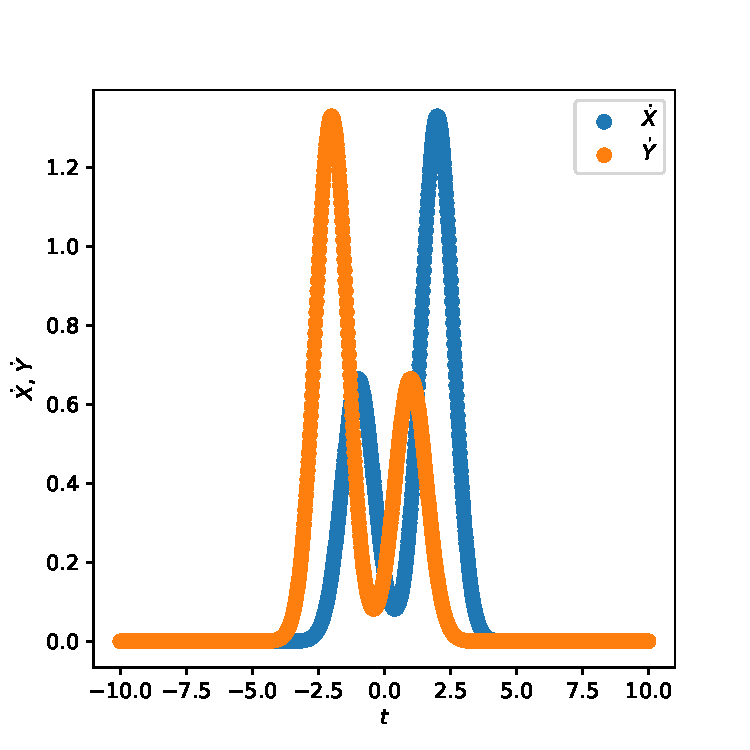
\includegraphics[width=0.32\textwidth]{exampleXdotYdot.pdf}
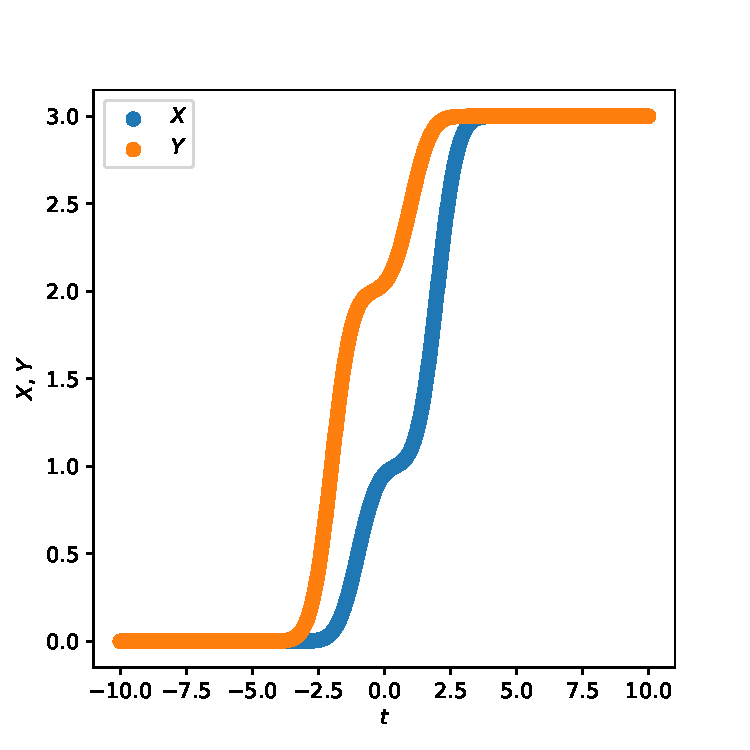
\includegraphics[width=0.32\textwidth]{exampleXY.pdf}
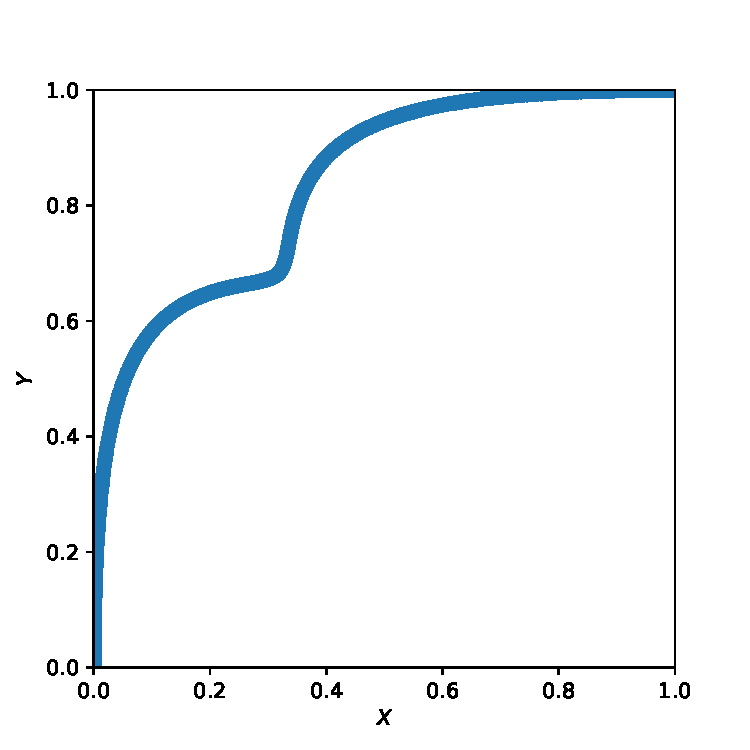
\includegraphics[width=0.32\textwidth]{exampleroc.pdf}
\caption{Plots for the example distributions.  Left: The density of non-responders \(\Xdot\) and responders \(\Ydot\).  Middle: The cumulative density of non-responders \(X\) and responders \(Y\).  Right: The ROC curve.\label{fig:exampledata}}
\end{center}
\end{figure}

We plug the differential equations \cref{eq:eulerlagrange_AUC} and boundary conditions \cref{eq:boundaryconditions,eq:boundaryconditions_AUC} into \texttt{scipy.integrate.solve\_bvp}.  For some range of \(\AUC\), this works pretty well.  We have to give it a decent starting guess for the curve and \(\Lambda\).  The way we do this is to start from the actual ROC curve (which is the solution when \(\AUC\) is the actual \(\AUC\) for \(x=X/n_X\) and \(y=Y/n_Y\)) and moving outwards in small increments.  Each time, the guess uses the fitted \(\Lambda\) and ROC curve, adjusted slightly to match the desired \(\AUC\), from the previous step.

There are two possible ways \texttt{solve\_bvp} can fail.  It can fail to converge, of course, but it can also converge on the following fake solution, which satisfies \cref{eq:eulerlagrange_AUC,eq:boundaryconditions,eq:boundaryconditions_AUC}:
\begin{align}
\begin{aligned}
x&=\Xdot/n_X \\
y&=\Ydot/n_Y \\
\Lambda&=0 \\
c_1&=2n_X \\
c_2&=2n_Y
\end{aligned}
\end{align}
In other words, \cref{eq:boundaryconditions_AUC} is a necessary but not sufficient replacement for \cref{eq:AUC}.  On the other hand, it may not matter so much, because \texttt{solve\_bvp} needs a decent guess anyway in order to converge.

A bigger issue is that beyond a certain point, \texttt{solve\_bvp} fails to converge even if we give it a guess based on an \(\AUC\) that is very close by.  A likelihood scan for \(\AUC\) in this example analysis within the range that works is shown in \cref{fig:examplelikelihoodscan}, together with the fitted values of \(\Lambda\), \(c_1\), and \(c_2\).

\begin{figure}
\begin{center}
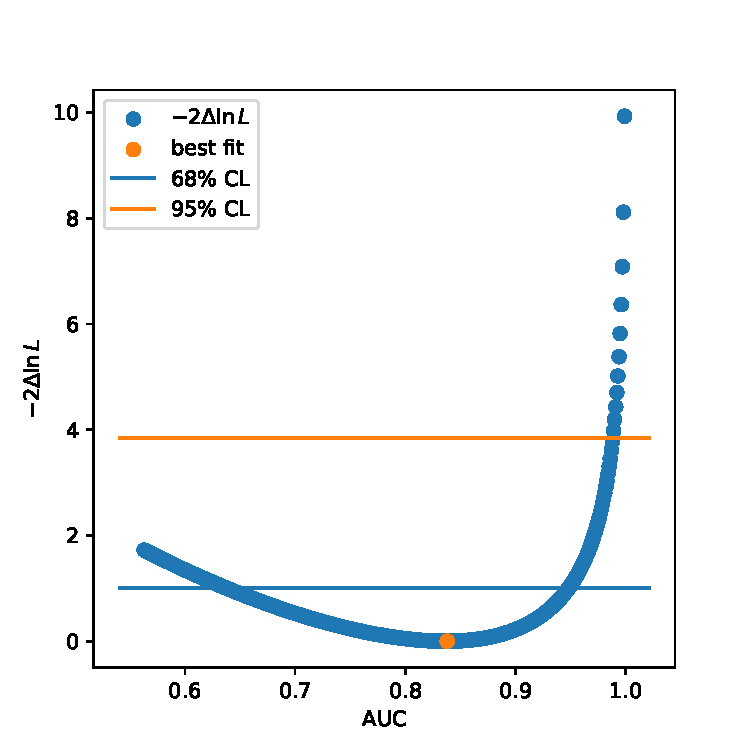
\includegraphics[width=0.32\textwidth]{examplescan.pdf}
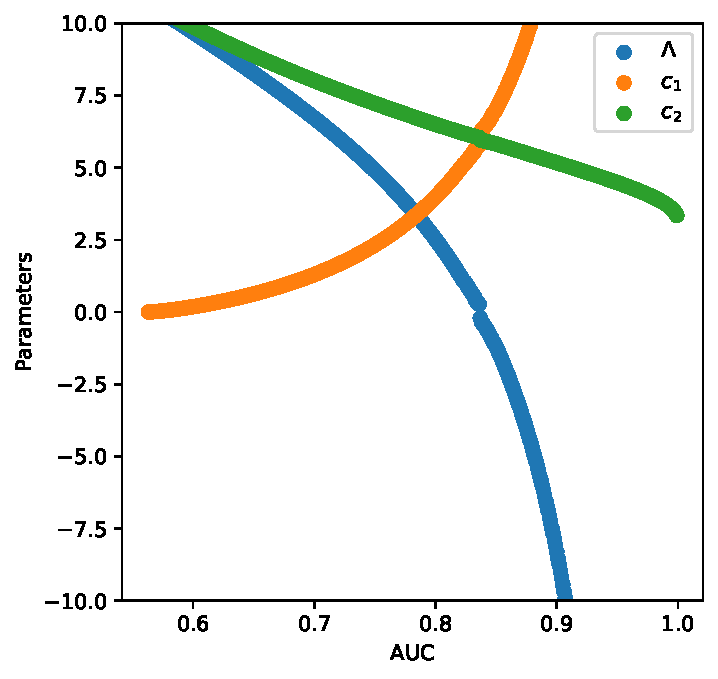
\includegraphics[width=0.32\textwidth]{exampleparameters.pdf}
\caption{Left: Likelihood scan for the \(\AUC\) using the example distributions.  Right: Fitted values of \(\Lambda\), \(c_1\), and \(c_2\) at each point in the likelihood scan.\label{fig:examplelikelihoodscan}}
\end{center}
\end{figure}

These plots go in steps of \(\Delta\AUC=\num{0.002}\) and down to \(\AUC=\num{0.564}\); by taking successively smaller steps, we can get down to \(\AUC=\num{0.55940501}\), where \(c_1=\num{6.36e-06}\).  Either \(c_1\) asymptotically goes to 0, in which case the issue might be numerical precision and a reparameterization could help, or there is some kind of phase transition and the solution jumps somewhere else in the space of possible ROC curves and parameters.

\subsection{Lagrangian approach with delta functions}

We can also construct a Lagrangian, as in \cref{sec:lagrangian}, with discrete data distributions as in \cref{sec:discrete}, by constructing \(\Xdot\) and \(\Ydot\) as a sum of \(\delta\) functions.  Probably some of the logic underlying calculus of variations isn't technically correct when \(\Xdot\) and \(\Ydot\) are not continuous, but it will likely work out anyway.
\begin{align}
\begin{aligned}
\Xdot(t)&=\sum_n \mathscr{X}_n\delta(t-t_n) \\
\Ydot(t)&=\sum_r \mathscr{Y}_r\delta(t-t_r) \label{eq:XdotYdotdelta}
\end{aligned}
\end{align}
\Cref{eq:eulerlagrange_AUC} gives \(\Xdot=0\implies\xdot=0\) and \(\Ydot=0\implies\ydot=0\), meaning that \(\xdot\) and \(\ydot\) are also \(\delta\) functions.

Mathematica gives a closed-form solution\footnote{Mathematica actually puts 1 for the lower limits of integration, but we can fold that into the constants and set it to \(-\infty\) to make it easier to deal with} to \cref{eq:eulerlagrange_AUC} in terms of integrals of \(\Xdot\) and \(\Ydot\):
\begin{align}
x(t)=c_4+c_2\int_{-\infty}^{t} dT &\exp\left[\int_{-\infty}^{T} d\tau \left(\frac{\Xdotdot(\tau)}{\Xdot(\tau)}-\frac{\Lambda\Ydot(\tau)}{2c_1-\Lambda (X(\tau)-Y(\tau))}\right) \right] \label{eq:eulerlagrange_AUC_mathematica_x} \\
y(t)=c_3+\frac{2}{c_2}\int_{-\infty}^{t} dT \frac{\Xdot(T)\Ydot(T)}{2c_1-\Lambda(X(T)-Y(T))} &\exp\left[ -\int_{-\infty}^{T} d\tau \left(\frac{\Xdotdot(\tau)}{\Xdot(\tau)}-\frac{\Lambda\Ydot(\tau)}{2c_1-\Lambda (X(\tau)-Y(\tau))}\right) \right] \label{eq:eulerlagrange_AUC_mathematica_y}
\end{align}
We can integrate the \(\Xdotdot/\Xdot\) term into \(\ln \Xdot\).  Because it's in an exponential, the lower limit of integration becomes a multiplicative constant \(k\), and we can fold it into \(c_5\equiv c_2k\).  This works in both \(x\) and \(y\), because \cref{eq:eulerlagrange_AUC_mathematica_x} has \(c_2\) in the numerator and a positive sign in front of the integral in the exponential, and \cref{eq:eulerlagrange_AUC_mathematica_y} has \(c_2\) in the denominator and a negative sign in front of the exponential.
\begin{align}
	x(t)=c_4+c_5\int_{-\infty}^{t} dT &\exp\left[\ln{\Xdot(T)}-\int_{-\infty}^{T} d\tau \left(\frac{\Lambda\Ydot(\tau)}{2c_1-\Lambda (X(\tau)-Y(\tau))}\right) \right] \label{eq:eulerlagrange_AUC_mathematica_x_simplify} \\
	y(t)=c_3+\frac{2}{c_5}\int_{-\infty}^{t} dT \frac{\Xdot(T)\Ydot(T)}{2c_1-\Lambda(X(T)-Y(T))} &\exp\left[ -\ln{\Xdot(T)}+\int_{-\infty}^{T} d\tau \left(\frac{\Lambda\Ydot(\tau)}{2c_1-\Lambda (X(\tau)-Y(\tau))}\right) \right] \label{eq:eulerlagrange_AUC_mathematica_y_simplify}
\end{align}

Now we plug in \cref{eq:XdotYdotdelta}:
\begin{align}
\begin{aligned}
x(t)=c_4+c_5\int_{-\infty}^{t} dT &\Xdot(T)\exp\left[-\sum_{\substack{r\\t_r<T}} \left(\frac{\Lambda\mathscr{Y}_r}{2c_1-\Lambda (X(t_r)-Y(t_r))}\right) \right] \\
    =c_4+c_5\sum_{\substack{n\\t_n<t}} &\mathscr{X}_n\exp\left[-\sum_{\substack{r\\t_r<t_n}} \left(\frac{\Lambda\mathscr{Y}_r}{2c_1-\Lambda (X(t_r)-Y(t_r))}\right) \right]
\end{aligned} \\
\begin{aligned}
y(t)=c_3+\frac{2}{c_5}\int_{-\infty}^{t} dT \frac{\Ydot(T)}{2c_1-\Lambda(X(T)-Y(T))} &\exp\left[\sum_{\substack{r\\t_r<T}} \left(\frac{\Lambda\mathscr{Y}_r}{2c_1-\Lambda (X(t_r)-Y(t_r))}\right) \right] \\
y(t)=c_3+\frac{2}{c_5}\sum_{\substack{r^\prime\\t_{r^\prime}<t}} \frac{\mathscr{Y}_{r^\prime}}{2c_1-\Lambda(X(t_{r^\prime})-Y(t_{r^\prime}))} &\exp\left[\sum_{\substack{r\\t_r<t_{r^\prime}}} \left(\frac{\Lambda\mathscr{Y}_r}{2c_1-\Lambda (X(t_r)-Y(t_r))}\right) \right]
\end{aligned}
\end{align}

We have five unknown parameters \((c_1, c_3, c_4, c_5, \Lambda)\) and five constraints \cref{eq:AUC,eq:boundaryconditions}, which we can solve using \texttt{scipy.optimize.fsolve}.

We plug in this solution and, for a simple enough ROC curve, get results that are 100\% in agreement with the solution from \cref{sec:discrete}.  \Cref{fig:exampledata_delta_functions_agreement} shows the likelihood scan and fitted ROC curve for responders \((-10, 0, 10)\) and non-responders \((-5, 5, 15)\).

For a more complicated ROC curve (\cref{fig:exampledata_delta_functions_disagreement}), the results are slightly different, and the calculated negative log likelihood is consistently higher using the \(\delta\) functions approach than using the discrete method.  Because the simple case in \cref{fig:exampledata_delta_functions_agreement} gives 100\% agreement, this is most likely a numerical issue in the solution using one of the methods.  Furthermore, we can conclude that the problem probably arises in the \(\delta\) functions solution, because when we optimize the log likelihood for a fixed \AUC, we can only incorrectly find a worse ROC curve, not a better one.  However, this deserves further investigation.

\begin{figure}
\begin{center}
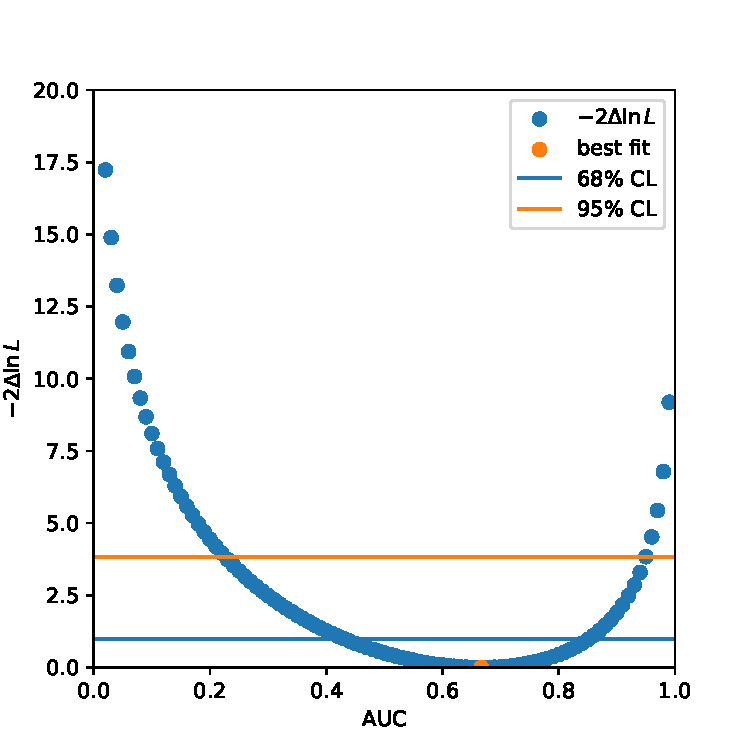
\includegraphics[width=0.32\textwidth]{deltafunctions_scan.pdf}
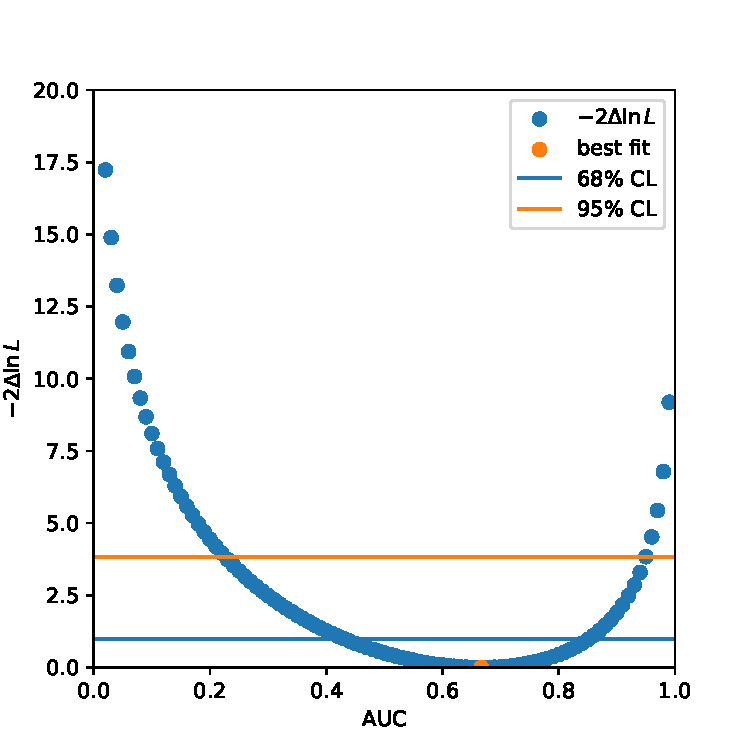
\includegraphics[width=0.32\textwidth]{discrete_scan_compare_to_delta_functions.pdf}
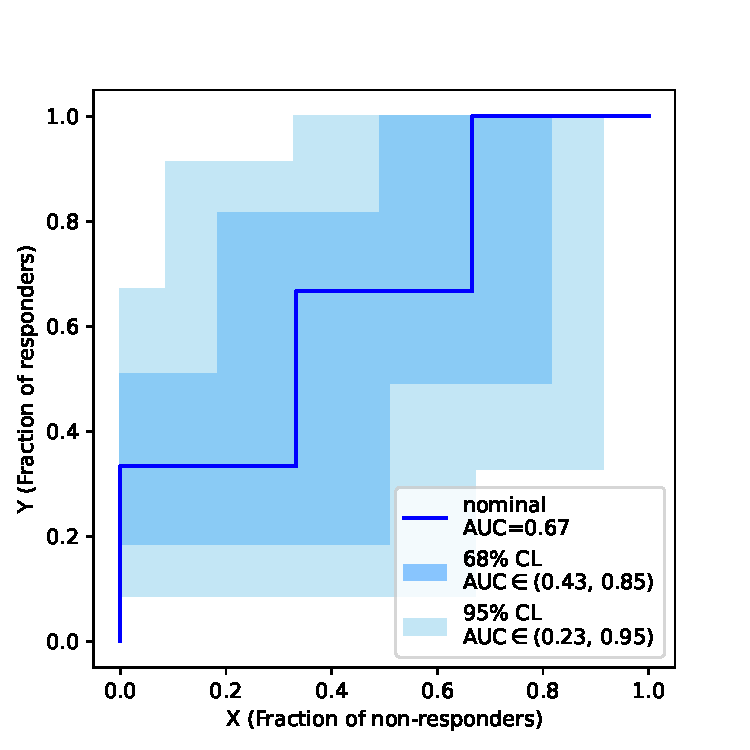
\includegraphics[width=0.32\textwidth]{deltafunctions_exampleroc_errors.pdf}
\caption{Left: Likelihood scan for the \(\AUC\) using the example distributions, using the Lagrangian approach with \(\delta\) functions.  Middle: Likelihood scan using the discrete method from \cref{sec:discrete}.  Right: The ROC curve with error bars.\label{fig:exampledata_delta_functions_agreement}}
\end{center}
\end{figure}

\begin{figure}
\begin{center}
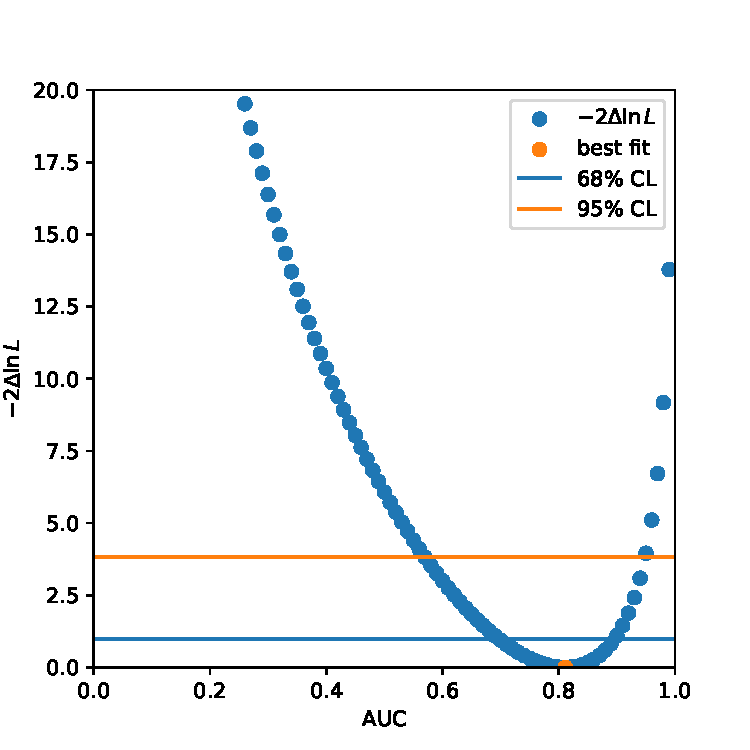
\includegraphics[width=0.32\textwidth]{discrete_scan.pdf}
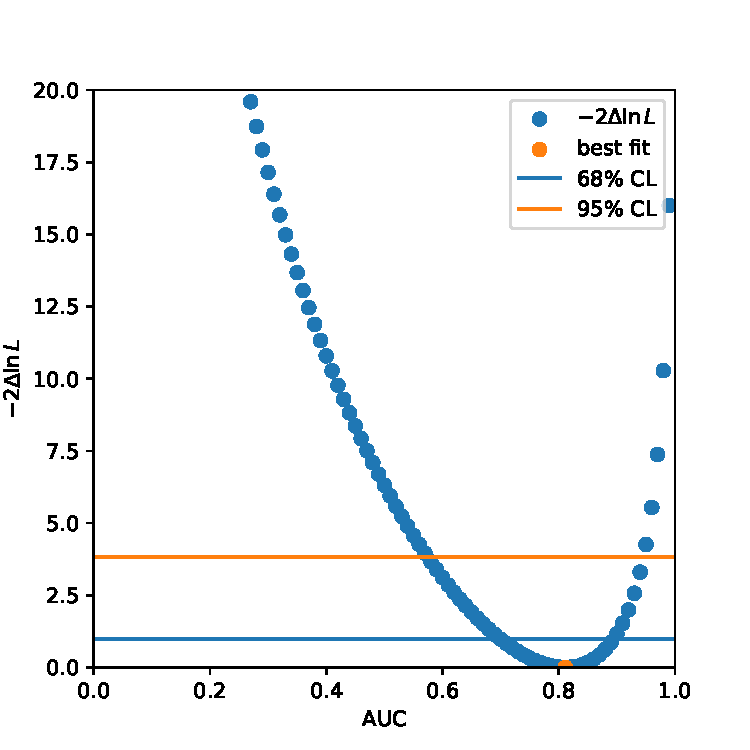
\includegraphics[width=0.32\textwidth]{delta_functions_scan_compare_to_discrete.pdf}
\caption{Left: Likelihood scan for the \(\AUC\) from \cref{fig:exampledata_discrete}.  Right: Likelihood scan using the Lagrangian approach with \(\delta\) functions.\label{fig:exampledata_delta_functions_disagreement}}
\end{center}
\end{figure}

\section{Incorporating systematic uncertainties}

Our ultimate goal is to incorporate systematic uncertainties into the methods described in the previous section.

To be more precise, the ``systematic'' uncertainties we consider here include every sample-by-sample uncertainty.  These include real systematic uncertainties, but also certain statistical uncertainties---for example, if our parameter \(t\) is a count or a ratio of counts, then they have Poisson uncertainties, and those would be included here.

\subsection{Monte Carlo method for systematics}

As a first step, we implemented error bands on ROC curves using \emph{only} systematic uncertainties, ignoring the binomial error that we dealt with in \cref{sec:stat}.  We use \(x=X\) and \(y=Y\), with the modification that we don't know exactly what \(X\) and \(Y\) are: they depend on the systematic uncertainties.

We model each responder and non-responder using a distribution of the systematic uncertainties, and generate a large sample of ROC curves from those distributions.  We then take percentiles of those ROC curves to estimate the 68\% and 95\% confidence intervals.

\Cref{fig:exampleroc_systematics_mc} shows example ROC curves calculated using this method.  They were previously presented as \autocite{SITC2023poster}, and are based on an analysis using CD8+FoxP3+ cells in non-small-cell lung cancer.  A higher density of these cells correlate with response to anti-PD1 immunotherapy, but the cells are quite rare and their count has a high Poisson uncertainty.  We also define ``CD8+FoxP3+-like neighborhoods'', which also correlate with response to treatment, but are much more common.  The two left plots show ROC curves based on the densities of CD8+FoxP3+ cells and CD8+FoxP3+-like neighborhoods, respectively.  Although the nominal \AUC's are almost the same, the plot using the rare CD8+FoxP3+ cells has a much larger error.

The right plot shows an example systematic uncertainty on the density of CD8+FoxP3+-like neighborhoods.  The uncertainty is estimated using the overlap region between two high-power fields of the microscope, which provide two independent measurements of a subset of the cells and is modeled using a log-normal distribution.  The systematic uncertainty is assumed to arise from residual errors after the flatfielding and lens corrections have been applied to the raw data from the microscope, and it is therefore modeled as 100\% correlated between different samples scanned in the same batch (which can include both responders and non-responders).

\begin{figure}
\begin{center}
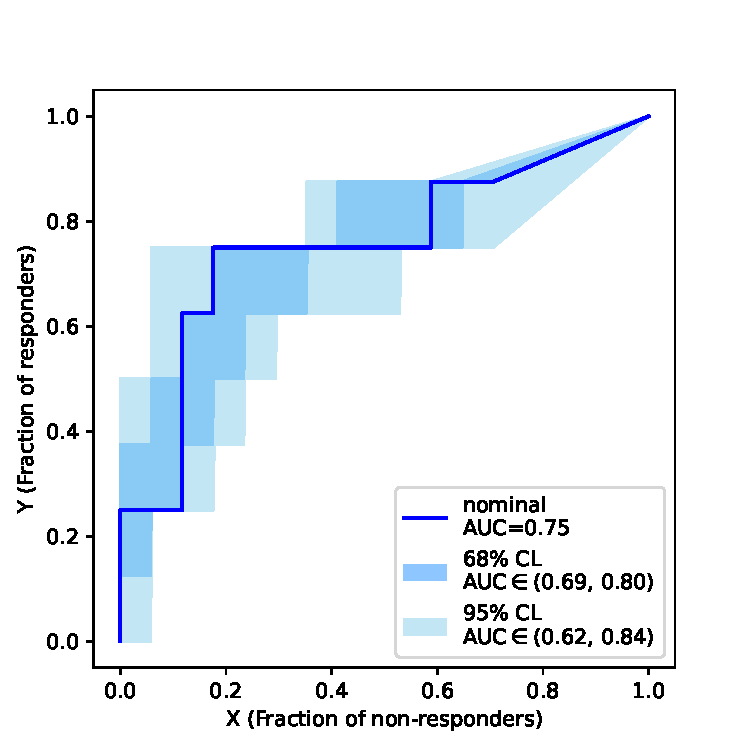
\includegraphics[width=0.32\textwidth]{poisson_roc_cells.pdf}
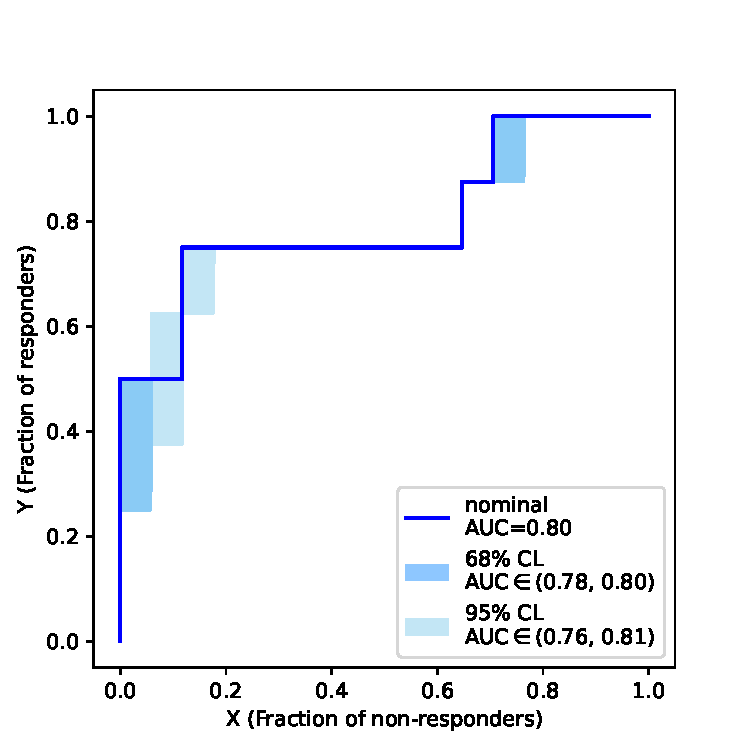
\includegraphics[width=0.32\textwidth]{poisson_roc_neighborhoods.pdf}
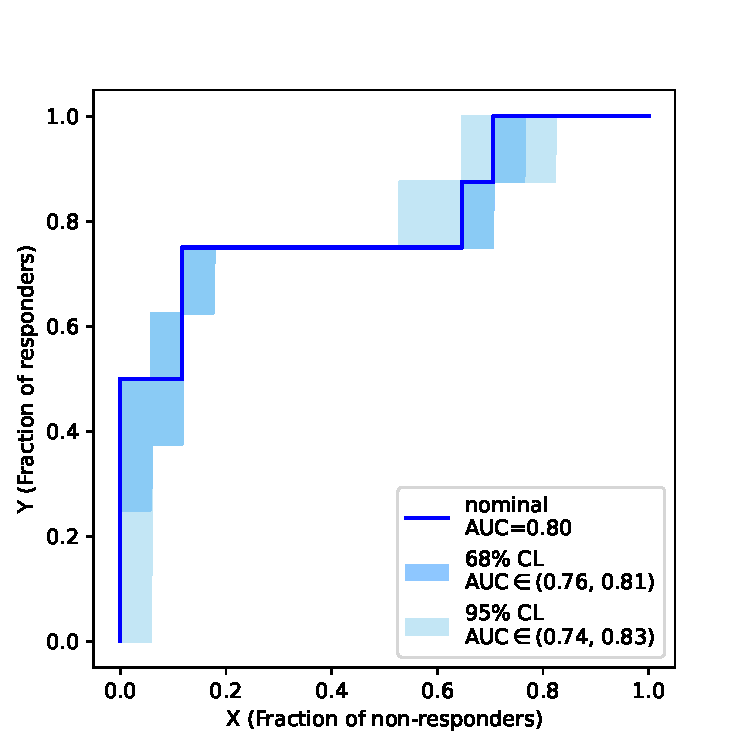
\includegraphics[width=0.32\textwidth]{lognormal_roc_neighborhoods.pdf}
\caption{ROC curves \autocite{SITC2023poster} showing the separation power of CD8+FoxP3+ cells (left) and CD8+FoxP3+-like neighborhoods (middle and right) to predict response to immunotherapy.  The \qty{68}{\%} and \qty{95}{\%} confidence bands on the ROC curves, coming from the Poisson error on the number of cells or neighborhoods (left and middle) and from the systematic error estimated using the overlap regions (right), are indicated.  The legends show the areas under the ROC curves (AUC) and their \qty{68}{\%} and \qty{95}{\%} confidence intervals.\label{fig:exampleroc_systematics_mc}}
\end{center}
\end{figure}

\section{Next steps}

\subsection{Discrete \texorpdfstring{\(\Xdot\)}{Xdot} and \texorpdfstring{\(\Ydot\)}{Ydot}, continuous \texorpdfstring{\(\xdot\)}{xdot} and \texorpdfstring{\(\ydot\)}{ydot}}
In reality, \(\Xdot\) and \(\Ydot\) should be \(\delta\) functions (they are in data, after all), and we can either make some assumptions on the form of \(\xdot\) and \(\ydot\) or add a term in the Lagrangian to help them behave nicely.  A physics analogy could lead to something like \(\frac{1}{2}m(\xdot^2+\ydot^2)\).

Once we do this, even the unconstrained Lagrangian (\cref{eq:lagrangian}) won't minimize at \(x=X/n_X, y=Y/n_Y\), but will probably be a smoothed version of that curve.

\subsection{Systematics}\label{sec:systematics}

The systematics will most likely go in the data distributions, so that \(\Xdot(t)\) and \(\Ydot(t)\) will become \(\Xdot(t,\vec{\beta})\) and \(\Ydot(t,\vec{\beta})\).  For example, let's say we have one sample at \(t=t_0\) with a log-normal systematic with a variation of \(1+\alpha\) at \(1\sigma\).  We will get
\begin{equation}
\Xdot(t,\beta)=\delta(t{(1+\alpha)}^{\beta}-t_0)
\end{equation}
and the Lagrangian will get a term
\begin{equation}
\mathcal{\tilde{L}_\beta}=\beta^2
\end{equation}

A sample will, in general, have multiple systematics, including log-normal and Poisson and probably others.  Some of the systematics will be correlated between a subset of the samples (for example, flatfielding and warping will be correlated between all samples in a batch).

\printbibliography{}
\end{document}
